\section{Linked Open Data (LOD) and the Web of Data concept}
Disambiguation of named entities by linking them with a knowledge base has many benefits that contribute in bringing the idea of Semantic Web of Data and the Linked Open Data principles closer to realization. Berners-Lee et al. \cite{lod_sofar} define \ac{lod} as follows: 

\begin{quote}
 "Linked Data is simply about using the Web to created typed links between data from different sources. It refers to data published on the Web in such a way that it is machine-readable, its meaning is explicitly defined, it is linked to other external data sets and can in turn be linked to and from other data sets.".\cite{lod_sofar}
\end{quote}

Furthermore, Tim Berners-Lee also argues that "\textit{The first step to semantic web is putting data on the web in a form that is understandable by machines or converting it to that form}" \cite{lod_sofar}. This is an important concept to shift our focus to, because it provides the means of publishing data on the web in such a way that all data published in the \ac{lod} will become part of a single global data space. The concept of Semantic Web should not be understood in alignment with the old and traditional "web of pages" where the main concern is putting data on the web. Semantic Web is about making links which should encourage exploration of the semantically connected web of data not only by humans but also by machines. Since the current WEB consists of large amount of unstructured information, based on the principles of \ac{lod} and Web of Data, it is necessary to convert this information to the desired form so that the goal of having a Semantic Web of Data is finally reached. "\textit{While semantic web, or web of data, is the goal for the end-result of this process, Linked Open Data provides the means to reach that goal}" \cite{lod_sofar}.

Our work contributes to the idea of semantic web and \ac{lod} principles in a way that it provides an effective and efficient way of semantically enriching unstructured web documents by disambiguation and linking the identified named entities with a \ac{kb} that is part of the \ac{lod} cloud (such as DBpedia) \cite{dbpedia}. Bauer et al. \cite{23} called Dbpedia "the semantic sister" of the most popular online encyclopedia in the world: Wikipedia, which makes Dbpedia one of the largest cross-domain knowledge bases extracted from the English edition of Wikipedia  \cite{23}. During the time of writing, Dbpedia is said to be the nucleus of the \ac{lod} cloud. It is one of the few \ac{kb} that has most in-links and out-links to other \ac{kb} published on the \ac{lod} cloud \cite{dbpedia, 23}. The so-called LOD-Cloud, covers more than an estimated 50 billion facts from many different domains like geography, multimedia, biology, politics, academia, energy and the like. Datasets published in the cloud are described with a unique language called "Resource Description Framework" or \ac{rdf} for short. It is a widely adopted standard for describing metadata as well as providing the means of structuring and linking data that describe things in the real world \cite{lod_sofar}. Figure \ref{fig:lod_diagram} represents the \ac{lod} Diagram as of 2017 and is constantly updated and maintained by the Linked Open Data initiative community \cite{lod-diagram}.

\begin{figure}[]
  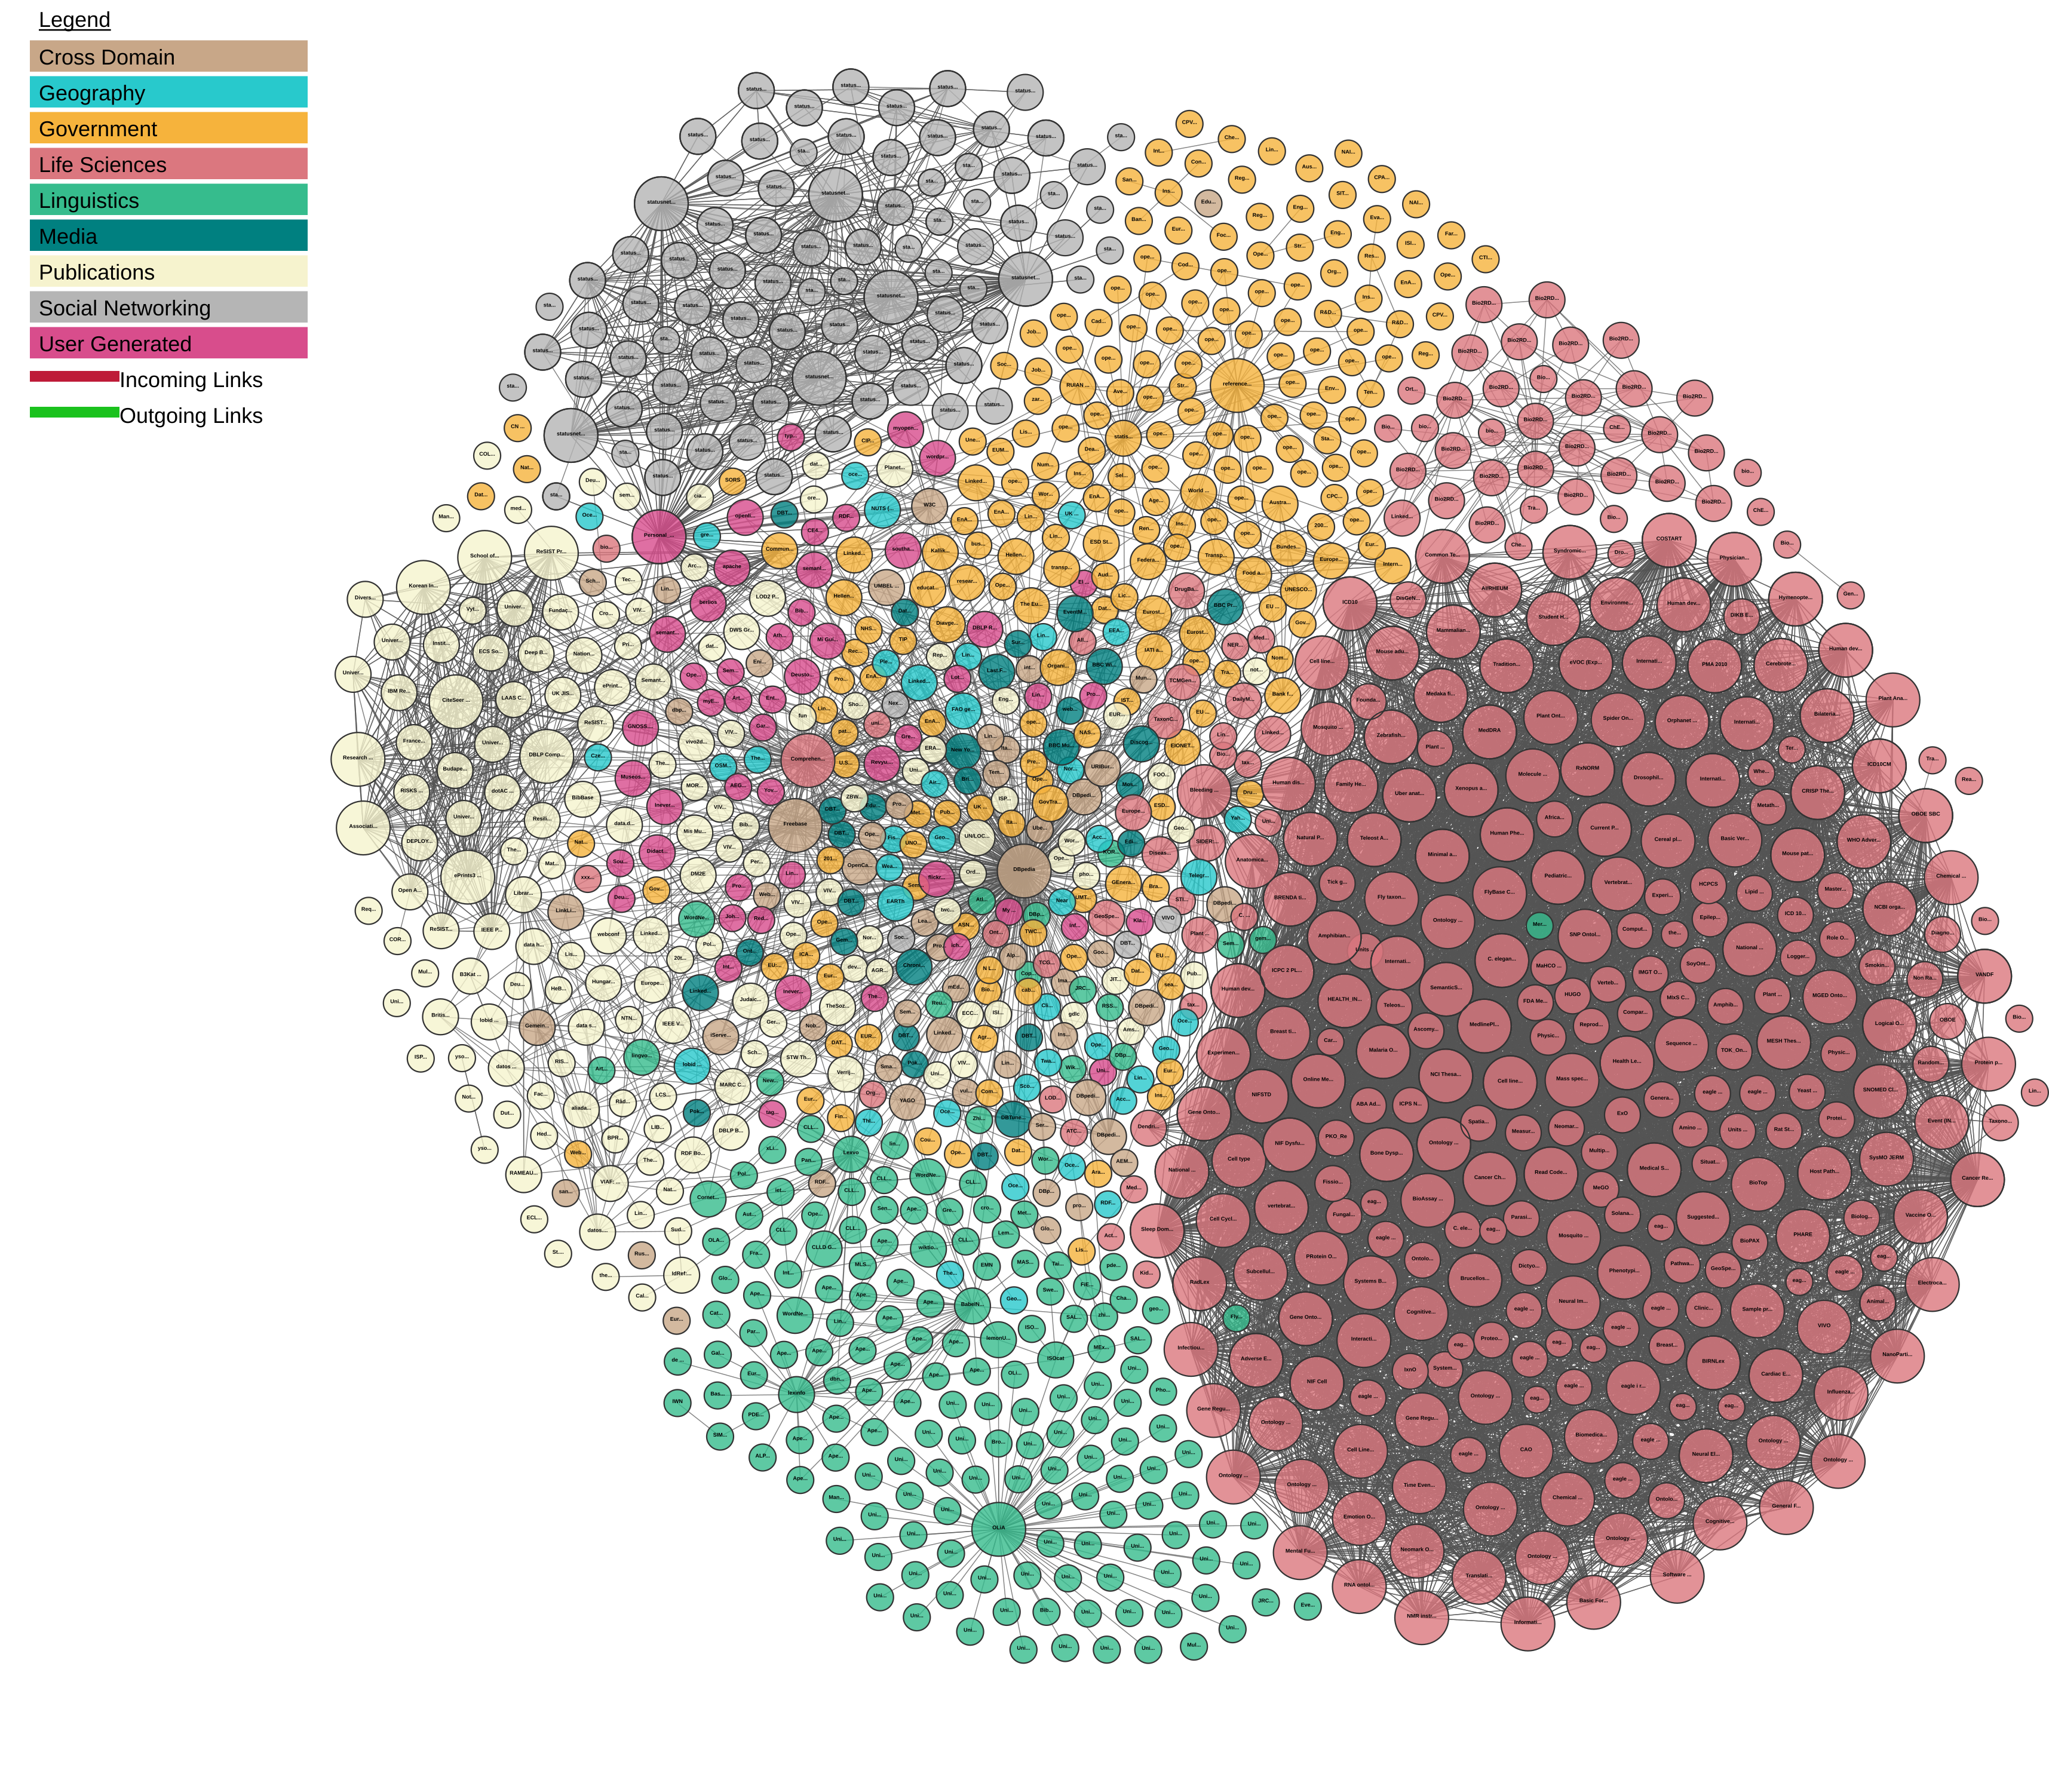
\includegraphics[width=\linewidth]{figures/lod.png}
  \caption{Linked Open Data cloud diagram 2017 \cite{lod-diagram}}
  \label{fig:lod_diagram}
\end{figure}
